
%%%%%%%%%%

\begin{frame}{\vskip -0.45cm \large Le probl\`eme d'optimisation derri\`ere les arbres de classification}

\small

\begin{multicols}{2}

	\begin{flushleft}
	\begin{minipage}{4.5cm}
	\vskip -0.5cm
	
%%%%%%%%%%

%\begin{figure}[h]

\centering
\begin{tikzpicture}

\node at (0,0) {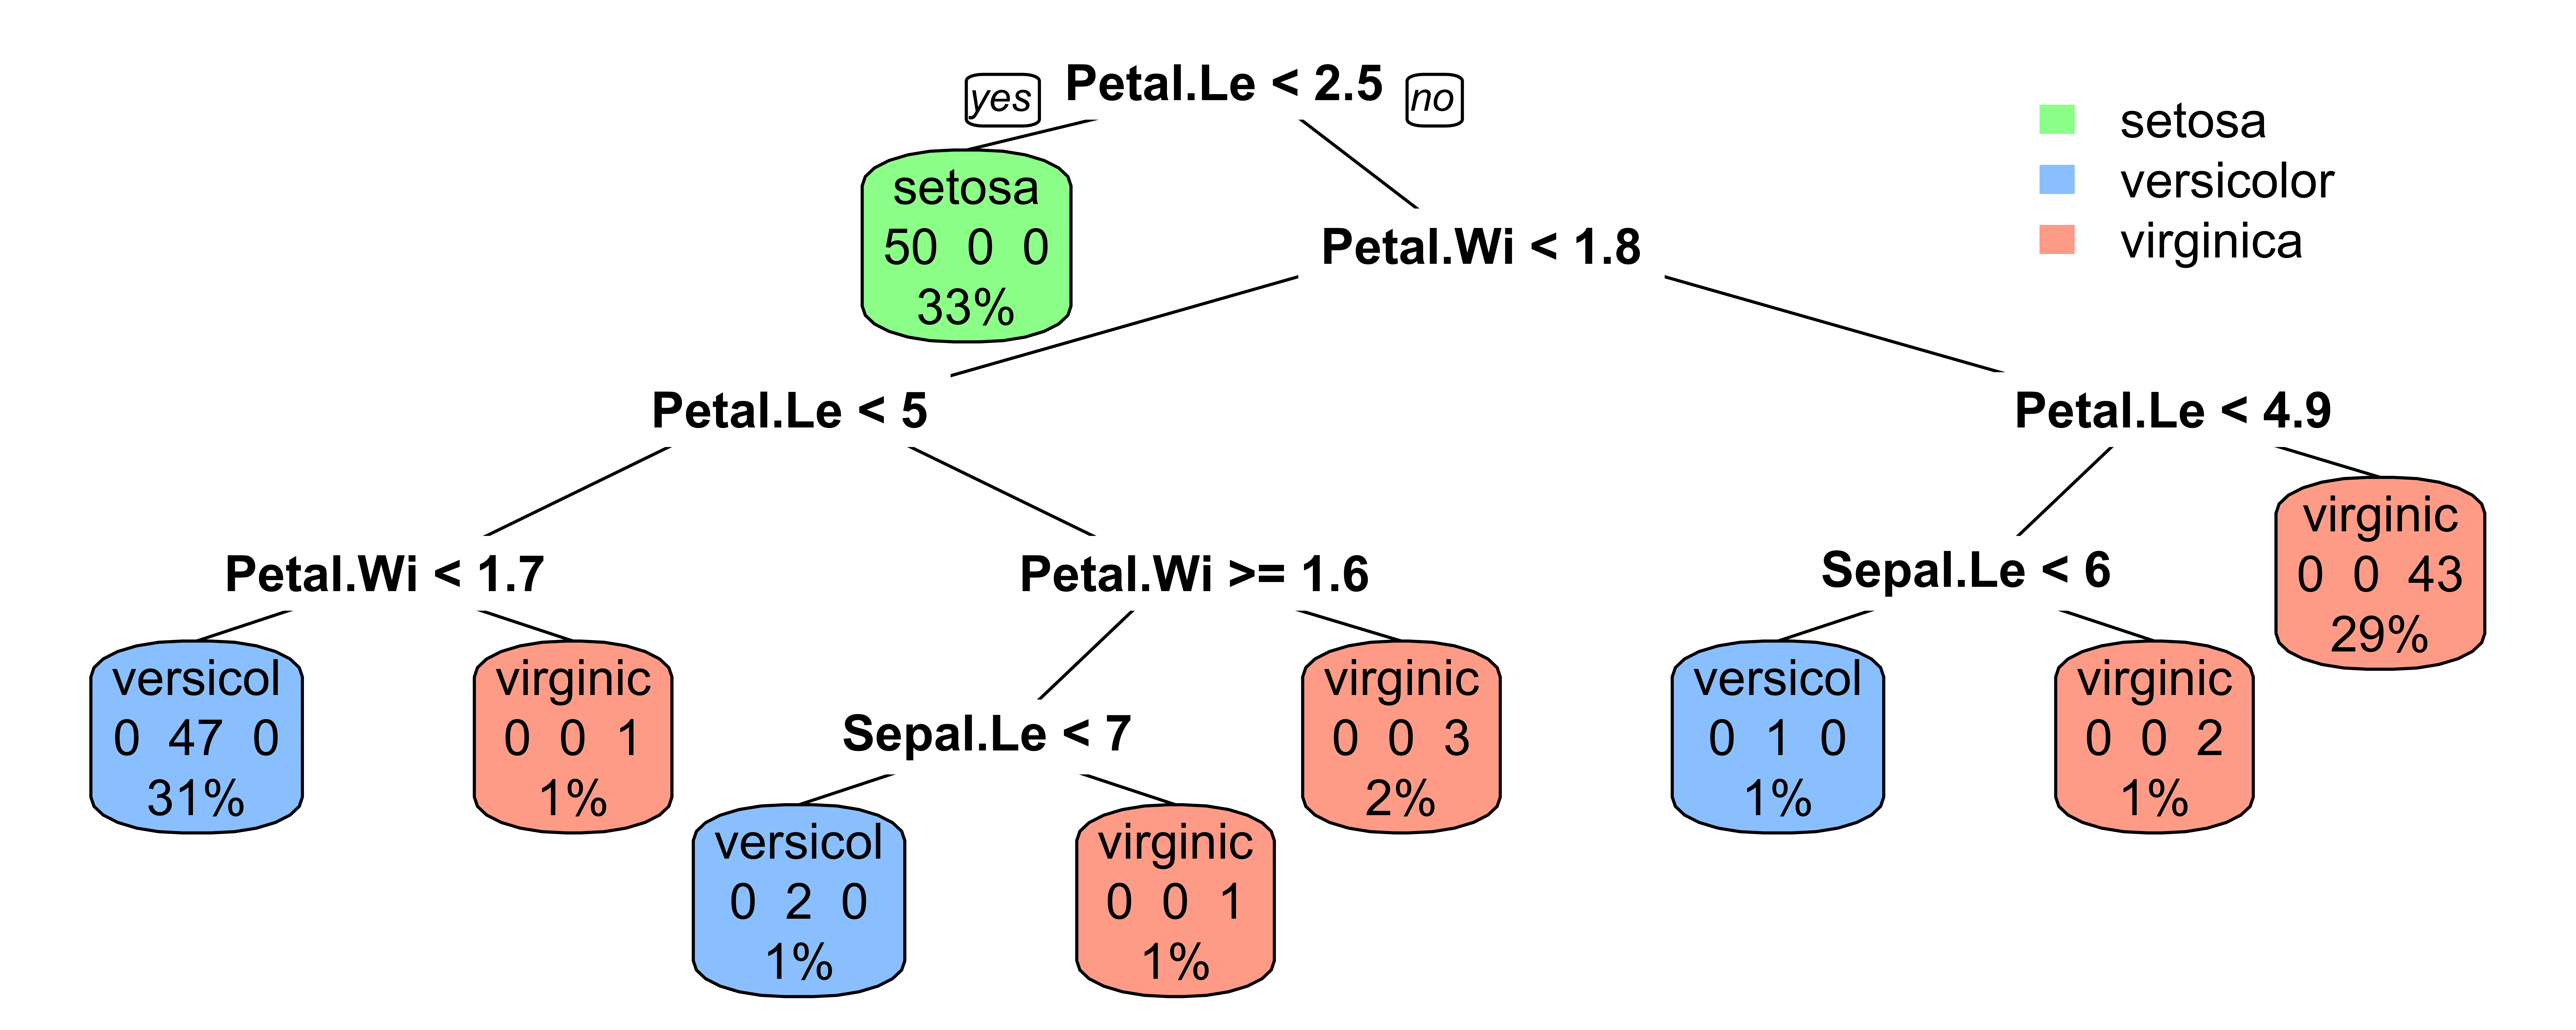
\includegraphics[width=4.5cm,height=6.25cm]{graphics/plot-rpart.png}};

%\node at (-1.55,-0.6) {\scriptsize$H(l_{1}\vert D) = 0$};
%\node at (-0.45,-3.125) {\scriptsize$H(l_{2}\vert D) = 0.445$};
%\node at (1.85,-3.125) {\scriptsize$H(l_{3}\vert D) = 0.151$};

%\node at (-1.55,-0.6) {\scriptsize$G(l_{1}\vert D) = 0$};
%\node at (-0.45,-3.125) {\scriptsize$G(l_{2}\vert D) \approx 0.168$};
%\node at (1.85,-3.125) {\scriptsize$G(l_{3}\vert D) \approx 0.043$};

\node at (-1.55,-0.675) {\scriptsize$G(l_{1}\vert D) = 0$};
\node at (-0.45,-3.15) {\scriptsize$G(l_{2}\vert D) \approx 0.168$};
\node at (1.85,-3.15) {\scriptsize$G(l_{3}\vert D) \approx 0.043$};

%%%  ~~~~~~~~~~  %%%

%%%%%%%%

\end{tikzpicture}

%%%%%%%%%%

	\end{minipage}
	\only<1-7|handout:0>{
		{\color{white}\scriptsize\begin{equation*}
		I(T \vert D) = \frac{50}{150}\times 0 + \frac{54}{150}\times 0.168 + \frac{46}{150} \times 0.043
		\end{equation*}}
		}
	\vskip -0.15cm
	\only<8->{
		{\scriptsize\begin{equation*}
		I(T \vert D) = \frac{{\color{red}50}}{150}\times 0 + \frac{{\color{red}54}}{150}\times 0.168 + \frac{{\color{red}46}}{150} \times 0.043
		\end{equation*}}
		}
	\end{flushleft}

\columnbreak

	\begin{flushright}
	\begin{minipage}{6.0cm}
	\vskip -0.6cm
	\pause
		{\Large Fonction objective}
	\pause
		\begin{center}\textbf{Impuret\'e d'arbres\\ d'apr\`es les donn\'ees}\end{center}
	\pause
		\begin{equation*}
		I(T\,\vert D)
		\; =
			\underset{l\,\in\,\textnormal{Feuilles}(T)}{\sum}\!\!
			P(X \!\in\! l\,) \cdot I(l\,\vert D)
		\end{equation*}
		{\scriptsize o\`u}
		{\scriptsize\begin{eqnarray*}
		\only<1-6|handout:0>{\color{white}
			P(X \!\in\! l\,) &\color{white}=& \color{white}\left(\!\!\!\begin{array}{c}
			\textnormal{probabilit\'e pour}
			\\
			\textnormal{une unit\'e tir\'ee au hasard}
			\\
			\textnormal{de parvenir la feuille $l$}
			\end{array}\!\!\!\!\right)
			}
		\only<7->{
			P(X \!\in\! l\,) &=& \left(\!\!\!\begin{array}{c}
			\textnormal{probabilit\'e pour}
			\\
			\textnormal{une unit\'e tir\'ee au hasard}
			\\
			\textnormal{de parvenir la feuille $l$}
			\end{array}\!\!\!\!\right)
			}
		\only<1-4|handout:0>{
		\\
			\color{white}I(l\,\vert D) &\color{white}=& \color{white}\left(\!\!\begin{array}{c}
				\textnormal{impurity of leaf $l$}
				\\
				\textnormal{given data $D$}
				\end{array}\!\!\right)
			}
		\only<5->{
		\\
			I(l\,\vert D) &=& \left(\!\!\begin{array}{c}
				\textnormal{impuret\'e de la feuille $l$}
				\\
				\textnormal{d'apr\`es les donn\'ees $D$}
				\end{array}\!\!\right)
			}
		\end{eqnarray*}}
	\pause
		\only<1-5|handout:0>{\color{white}\begin{center}
		\vskip -0.5cm
		{\scriptsize Choix communs pour $I(l\,\vert D)$:}
		\vskip 0.1cm
		Entropy ($H$),\;
		Gini Impurity ($G$)
		\end{center}}
		\only<6->{\begin{center}
		\vskip -0.5cm
		{\scriptsize Choix communs pour $I(l\,\vert D)$:}
		\vskip 0.1cm
		Entropie ($H$),\;
		Impuret\'e de Gini ($G$)
		\end{center}}
	\end{minipage}
	\end{flushright}

\end{multicols}

\end{frame}
\normalsize

%%%%%%%%%%

\begin{frame}{\vskip -0.2cm \Large Mesures d'impuret\'e : Entropie \& Impuret\'e Gini}

\vskip -0.2cm
\tiny
\begin{equation*}
I(l\,\vert D)
\;\; = \;\;
\left\{\begin{array}{ccl}
\textnormal{Entropie}
& := &
	\textnormal{\tiny$-\;\overset{C}{\underset{y=1}{\sum}}\;\,
	\widehat{p}(Y=c\,\vert X\in l\,) \cdot \log\,\widehat{p}(Y=c\,\vert X\in l\,)$}
\\
\textnormal{Impuret\'e de Gini}
& := &
	\textnormal{\tiny$+\;\overset{C}{\underset{y=1}{\sum}}\;\,
	\widehat{p}(Y=c\,\vert X\in l\,) \cdot
	\left(\overset{{\color{white}.}}{1}\,-\,\widehat{p}(Y=c\,\vert X\in l\,)\right)$}
\end{array}\right.
\end{equation*}

\begin{multicols}{2}

	\begin{minipage}{4.5cm}
	\begin{flushleft}
	\vskip 0.25cm
	{\scriptsize
	\begin{eqnarray*}
	\pause
	&&
		\textnormal{\normalsize$G\!\left(\left(\frac{0}{54},\frac{49}{54},\frac{5}{54}\right)\right)$}
	\\
	\pause
	& = &
		{\color{white}+} \;\frac{\overset{{\color{white}1}}{0}}{54} \cdot \left( 1 - \frac{0}{54} \right)
	\\
	&&
		+ \;\frac{49}{54} \cdot \left( 1 - \frac{49}{54} \right)
	\\
	&&
		+ \;\frac{5}{54} \cdot \left( 1 - \frac{5}{54} \right)
	\\
	\pause
	& \approx &
		\overset{{\color{white}-}}{\textnormal{\normalsize$0.168$}}
	\end{eqnarray*}
	}
	\end{flushleft}
	\end{minipage}
	
\columnbreak

	\pause
	\begin{minipage}{4.5cm}
	\begin{flushright}
	{\normalsize
	\begin{tabular}{|c|c|c|}
	\hline
	{\small Distribution} && {\small Gini} \\
	\hline \hline
	$({\color{gcblue}0.0}, 1.0)$ & \textnormal{\tiny$2(0.0)(1-0.0)$} & 0 \\
	$({\color{gcblue}0.1}, 0.9)$ & \textnormal{\tiny$2(0.1)(1-0.1)$} & 0.18 \\
	$({\color{gcblue}0.2}, 0.8)$ & \textnormal{\tiny$2(0.2)(1-0.2)$} & 0.32 \\
	$({\color{gcblue}0.3}, 0.7)$ & \textnormal{\tiny$2(0.3)(1-0.3)$} & 0.42 \\
	$({\color{gcblue}0.4}, 0.6)$ & \textnormal{\tiny$2(0.4)(1-0.4)$} & 0.48 \\
	$({\color{gcblue}0.5}, 0.5)$ & \textnormal{\tiny$2(0.5)(1-0.5)$} & 0.50 \\
	$({\color{gcblue}0.6}, 0.4)$ & \textnormal{\tiny$2(0.6)(1-0.6)$} & 0.48 \\
	$({\color{gcblue}0.7}, 0.3)$ & \textnormal{\tiny$2(0.7)(1-0.7)$} & 0.42 \\
	$({\color{gcblue}0.8}, 0.2)$ & \textnormal{\tiny$2(0.8)(1-0.8)$} & 0.32 \\
	$({\color{gcblue}0.9}, 0.1)$ & \textnormal{\tiny$2(0.9)(1-0.9)$} & 0.18 \\
	$({\color{gcblue}1.0}, 0.0)$ & \textnormal{\tiny$2(1.0)(1-1.0)$} & 0      \\
	\hline
	\end{tabular}
	}
	\end{flushright}
	\end{minipage}
	
\end{multicols}

\end{frame}
\normalsize

%%%%%%%%%%

\begin{frame}{\vskip -0.2cm \Large Mesures d'impuret\'e : Entropie \& Impuret\'e Gini}

\vskip -0.2cm
\tiny
\begin{equation*}
I(l\,\vert D)
\;\; = \;\;
\left\{\begin{array}{ccl}
\textnormal{Entropie}
& := &
	\textnormal{\tiny$-\;\overset{C}{\underset{y=1}{\sum}}\;\,
	\widehat{p}(Y=c\,\vert X\in l\,) \cdot \log\,\widehat{p}(Y=c\,\vert X\in l\,)$}
\\
\textnormal{Impuret\'e de Gini}
& := &
	\textnormal{\tiny$+\;\overset{C}{\underset{y=1}{\sum}}\;\,
	\widehat{p}(Y=c\,\vert X\in l\,) \cdot
	\left(\overset{{\color{white}.}}{1}\,-\,\widehat{p}(Y=c\,\vert X\in l\,)\right)$}
\end{array}\right.
\end{equation*}

\begin{multicols}{2}

	\begin{minipage}{4.5cm}
	\begin{flushright}
	\includegraphics[height=5.9cm]{graphics/plot-impurity-metrics.png}
	\end{flushright}
	\end{minipage}

\columnbreak

	\begin{minipage}{4.5cm}
	\begin{flushright}
	{\normalsize
	\begin{tabular}{|c|c|c|}
	\hline
	{\small Distribution} && {\small Gini} \\
	\hline \hline
	$({\color{gcblue}0.0}, 1.0)$ & \textnormal{\tiny$2(0.0)(1-0.0)$} & 0 \\
	$({\color{gcblue}0.1}, 0.9)$ & \textnormal{\tiny$2(0.1)(1-0.1)$} & 0.18 \\
	$({\color{gcblue}0.2}, 0.8)$ & \textnormal{\tiny$2(0.2)(1-0.2)$} & 0.32 \\
	$({\color{gcblue}0.3}, 0.7)$ & \textnormal{\tiny$2(0.3)(1-0.3)$} & 0.42 \\
	$({\color{gcblue}0.4}, 0.6)$ & \textnormal{\tiny$2(0.4)(1-0.4)$} & 0.48 \\
	$({\color{gcblue}0.5}, 0.5)$ & \textnormal{\tiny$2(0.5)(1-0.5)$} & 0.50 \\
	$({\color{gcblue}0.6}, 0.4)$ & \textnormal{\tiny$2(0.6)(1-0.6)$} & 0.48 \\
	$({\color{gcblue}0.7}, 0.3)$ & \textnormal{\tiny$2(0.7)(1-0.7)$} & 0.42 \\
	$({\color{gcblue}0.8}, 0.2)$ & \textnormal{\tiny$2(0.8)(1-0.8)$} & 0.32 \\
	$({\color{gcblue}0.9}, 0.1)$ & \textnormal{\tiny$2(0.9)(1-0.9)$} & 0.18 \\
	$({\color{gcblue}1.0}, 0.0)$ & \textnormal{\tiny$2(1.0)(1-1.0)$} & 0      \\
	\hline
	\end{tabular}
	}
	\end{flushright}
	\end{minipage}

\end{multicols}

\end{frame}
\normalsize

%%%%%%%%%%

\begin{frame}{\vskip -0.5cm \normalsize Fonction Objective : \vskip 0.05cm \Large l'Impuret\'e d'arbres d'apr\`es les donn\'ees}

\vskip -0.5cm

\begin{eqnarray*}
%\pause
I(T\,\vert D)
& = &
	\!\!\!\!
	\underset{l\,\in\,\textnormal{Feuilles}(T)}{\sum}\!\!
	{\color{red}P(X \!\in\! l\,)} \cdot I(l\,\vert D)
\\
%\pause
& \approx &
	\!\!\!\!
	\underset{l\,\in\,\textnormal{Feuilles}(T)}{\sum}
	{\color{red}\widehat{p}(X \!\in\! l\,)} \cdot I(l\,\vert D)
%\pause
\;\; = \;\;
	\!\!\!\!
	\underset{l\in\textnormal{Feuilles}(T)}{\sum}
	{\color{red}\dfrac{\overset{n}{\underset{i=1}{\sum}}\,I_{\{x_{i} \in l\}}}{n}} \cdot I(l\,\vert D)
\end{eqnarray*}

\small
\begin{equation*}
%\pause
I(l\,\vert D)
\; = \;
\left\{\begin{array}{ccl}
%\pause
\textnormal{Entropie}
& := &
	\textnormal{\scriptsize$-\;\overset{C}{\underset{y=1}{\sum}}\;\,
	\widehat{p}(Y=c\,\vert X\in l\,) \cdot \log\,\widehat{p}(Y=c\,\vert X\in l\,)$}
\\
%\pause
\textnormal{Impuret\'e de Gini}
& := &
	\textnormal{\scriptsize$+\;\overset{C}{\underset{y=1}{\sum}}\;\,
	\widehat{p}(Y=c\,\vert X\in l\,) \cdot
	\left(\overset{{\color{white}.}}{1}\,-\,\widehat{p}(Y=c\,\vert X\in l\,)\right)$}
\end{array}\right.
\end{equation*}

%\pause
\vskip -0.5cm

\footnotesize
\begin{equation*}
\widehat{p}(Y=c\,\vert X\in l\,)
\;\; := \;\;
	\left.\overset{n}{\underset{i=1}{\sum}}\; I_{\{x_{i}\in l, y_{i} = c\}} \right\slash
	\overset{n}{\underset{i=1}{\sum}}\; I_{\{x_{i}\in l\}}
\end{equation*}

\end{frame}
\normalsize

%%%%%%%%%%
